\documentclass[oneside,12pt,letterpaper]{article}

% Imports and Definitions
%% Packages
\usepackage{amsmath}
\usepackage{amsfonts}
\usepackage{amssymb}
\usepackage{amsthm}
\usepackage{arydshln}
\usepackage{color}
\usepackage{extramarks}
\usepackage{fancyhdr}
\usepackage{float}
\usepackage[margin=1in]{geometry}
\usepackage{graphicx}
\usepackage{listings}
\usepackage{multicol}
\usepackage{setspace}
\usepackage{subcaption}
\usepackage{textcomp}
\usepackage{url}
\usepackage{xspace}
\usepackage{mathtools}

%% Commands
%%% Metadata
\newcommand{\metaTitle}{Comprehensive Exam}
\newcommand{\metaDueDate}{November 24, 2020}
\newcommand{\metaDueTime}{04:00 PM}
\newcommand{\metaSchool}{IUPUI}
\newcommand{\metaClass}{STAT 52400}
\newcommand{\metaDepartment}{Statistics Department}
\newcommand{\metaAuthorName}{Ross Grinvalds}

%%% Aliases
\newcommand{\Bias}{\mathrm{Bias}}
\newcommand{\Cov}{\mathrm{Cov}}
\newcommand{\dd}[1]{\frac{\mathrm{d}}{\mathrm{d}x} (#1)}
\newcommand{\dx}{\mathrm{d}x}
\newcommand{\E}{\mathrm{E}}
\newcommand{\m}[1]{\begin{bmatrix*}[r]#1\end{bmatrix*}}
\newcommand{\md}[1]{\begin{vmatrix*}#1\end{vmatrix*}}
\newcommand{\mf}[1]{\mathrm{\bf{#1}}}
\newcommand{\p}[1]{\begin{pmatrix}#1\end{pmatrix}} 
\newcommand{\pdd}[2]{\frac{\partial}{\partial #1} (#2)}
\newcommand{\solution}{\textbf{\large Solution}}
\newcommand{\T}{\intercal}
\newcommand{\Var}{\mathrm{Var}}

%%% Math Functions
\makeatletter
\newsavebox{\mybox}\newsavebox{\mysim}
\newcommand{\distras}[1]{%
  \savebox{\mybox}{\hbox{\kern3pt$\scriptstyle#1$\kern3pt}}%
  \savebox{\mysim}{\hbox{$\sim$}}%
  \mathbin{\overset{#1}{\kern\z@\resizebox{\wd\mybox}{\ht\mysim}{$\sim$}}}%
}
\makeatother

\newcommand{\indep}{\perp \!\!\! \perp}

%% Environments
%%% R Code
\newcommand{\ri}[1]{\lstinline{#1}}  %% Short for 'R inline'

\lstnewenvironment{rc}[1][]{
	\lstset{commentstyle=\color{red}, keywordstyle=\color{black}, showstringspaces=true, language=R, basicstyle=\ttfamily\tiny}
}{}
\lstset{language=R}


% Settings
%% Document-wide
\pagestyle{fancy}

%% Header and Footer
\setlength{\headheight}{15pt}
\lhead{\metaAuthorName}
\chead{\metaSchool\ \metaClass:\ \metaTitle}
\rhead{\metaDepartment}
\cfoot{\thepage}

%% Title Page
\title{
	\vspace{1in}
	\textmd{\textbf{\metaSchool\ \metaClass:\ \metaTitle}}\\
	\normalsize\vspace{0.1in}\small{Due\ by\ \metaDueDate\ at \metaDueTime}\\
	\vspace{6in}
}
\author{\metaAuthorName}
\date{}


\begin{document}
\maketitle

\section*{Part 1} 
	This project focuses on the famous `iris' dataset. The data contains four independent variables including sepal length, sepal width, petal length, and petal width for three different species, setosa, versicolor, and virginica. A total of 150 observations were collected. Before performing any multivariate analysis, it is important to explore the data and assess the univariate and multivariate distribution of each of the independent variables. The key focus is to identify if the univariate and multivariate distributions of the data exhibit a normal tendency, however, it is also important to note that each of the different populations consist of 50 observations, allowing for large sample results to guide the analysis where needed.

Throughout Part I, only sepal length and sepal width will be considered for the analysis. Then, the univariate and bivariate normality of the data can be inspected for each of the three species using visual and statistical analysis. For each of the three populations, the spread of the data can be observed via a histogram and the normality observed via a quantile-quantile plot. These plots are ordered in pairs for the species setosa, versicolor, and virginica, respectively. Additionally, a Shapiro-Wilks test and a correlation coefficient test were performed for each of sepal length and sepal width for each of the species. In all cases, there is no reasonable evidence of a departure from normality.

\begin{center}
	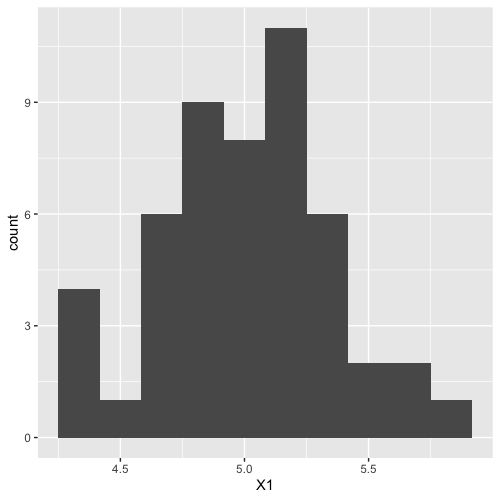
\includegraphics[width=1.5in]{I_1_X1_hist.png}
	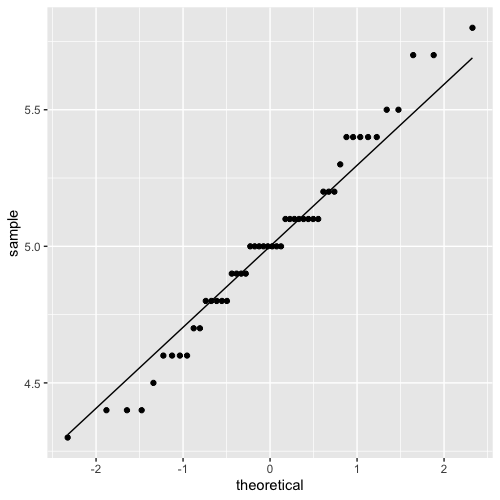
\includegraphics[width=1.5in]{I_1_X1_qq.png}
	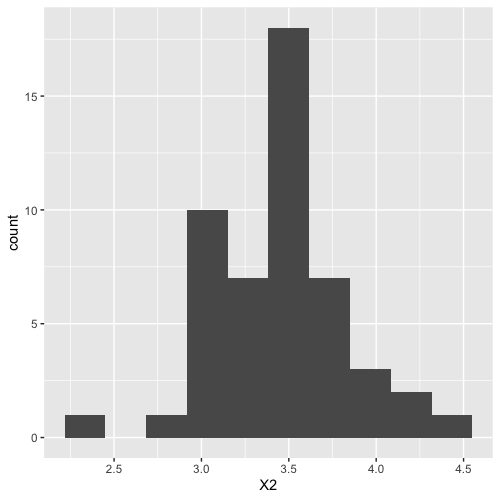
\includegraphics[width=1.5in]{I_1_X2_hist.png}
	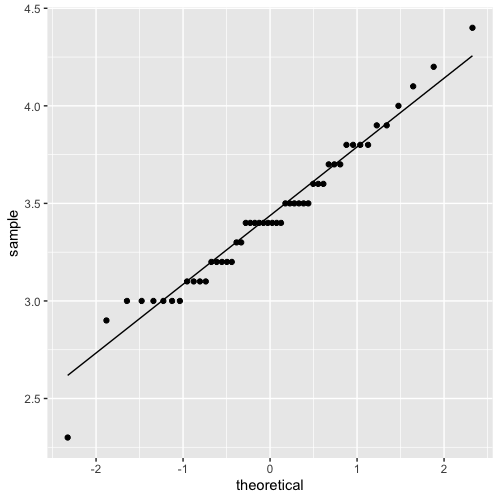
\includegraphics[width=1.5in]{I_1_X2_qq.png}
\end{center}
\begin{center}
	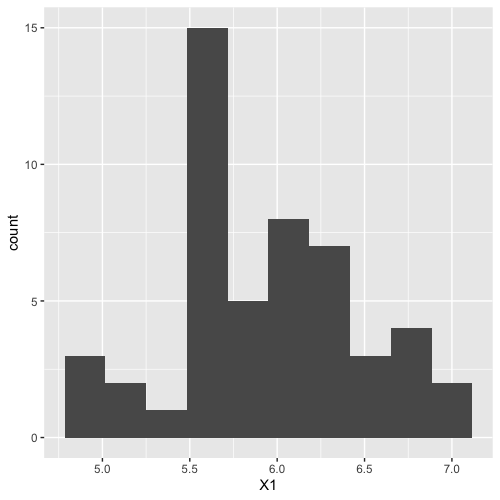
\includegraphics[width=1.5in]{I_2_X1_hist.png}
	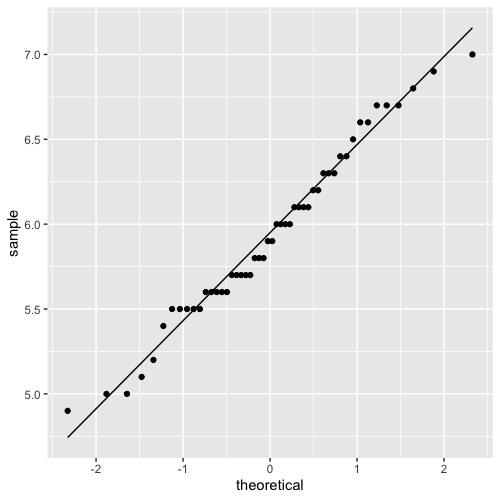
\includegraphics[width=1.5in]{I_2_X1_qq.png}
	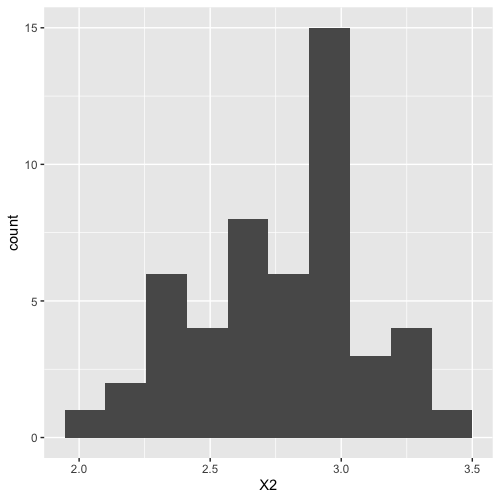
\includegraphics[width=1.5in]{I_2_X2_hist.png}
	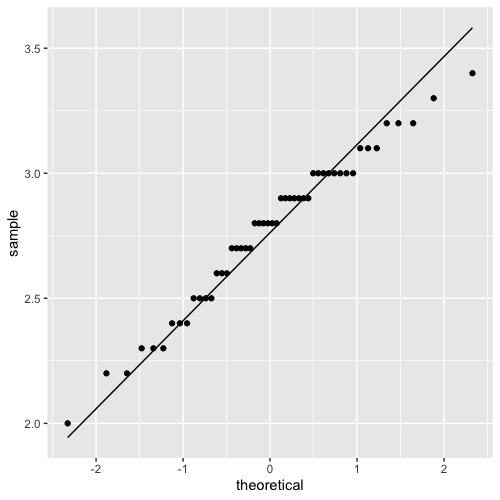
\includegraphics[width=1.5in]{I_2_X2_qq.png}
\end{center}
\begin{center}
	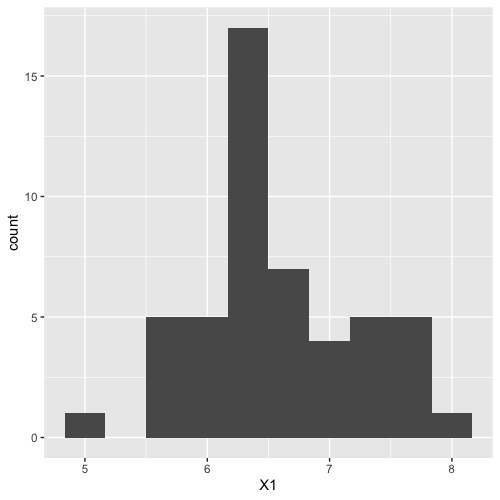
\includegraphics[width=1.5in]{I_3_X1_hist.png}
	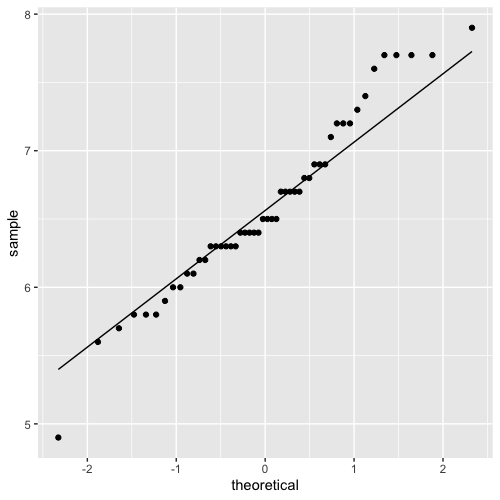
\includegraphics[width=1.5in]{I_3_X1_qq.png}
	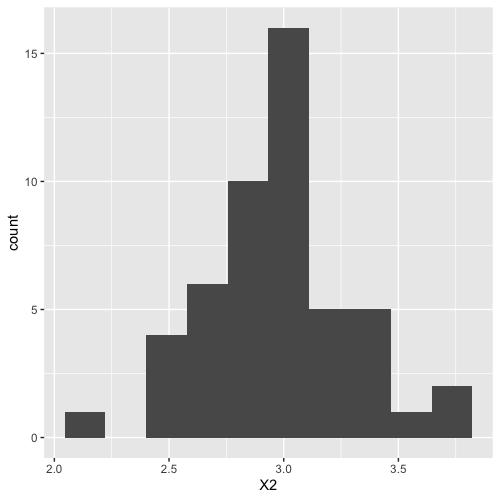
\includegraphics[width=1.5in]{I_3_X2_hist.png}
	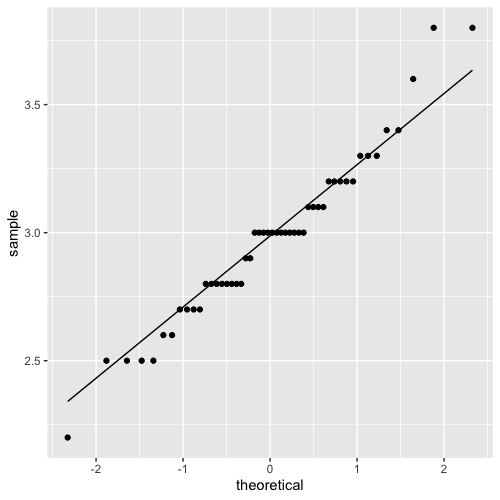
\includegraphics[width=1.5in]{I_3_X2_qq.png}
\end{center}

\begin{center}
\begin{tabular}{| c c | c c | c c |} 
	\hline
	group & variable & Shapiro-Wilks & p-value & correlation test & p-value \\
	\hline
	&&&&&\\
	setosa & length &  0.977 & 0.459 & 0.990 & 0.539\\
	& width &  0.971 & 0.271 & 0.981 & 0.125\\
	&&&&&\\
	versicolor & length &  0.977 & 0.464 & 0.991 & 0.623\\
	& width &  0.974 & 0.338 & 0.988 & 0.347\\
	&&&&&\\
	virginica & length &  0.971 & 0.258 & 0.985 & 0.220\\
	& width &  0.967 & 0.180 & 0.982 & 0.115\\
	&&&&&\\
	\hline
\end{tabular}
\end{center}

After the univariate analysis, the bivariate distribution of the data can be examined using visual and statistical measures. In terms of a visual aid, a scatterplot matrix, colored by species, provides a simple but intuitive measure for the spread of the data. There are several points in the data that seem to depart from the cloud of points, however, it isn't clear from this aid alone if these points are outliers. A second visual aid is the generalized distance plot that is a generalization of the quantile-quantile plot. A threshold of $\alpha=0.005$ is set as a cut-off to identify potential outliers. None of the generalized distances exceed the threshold.

\begin{center}
	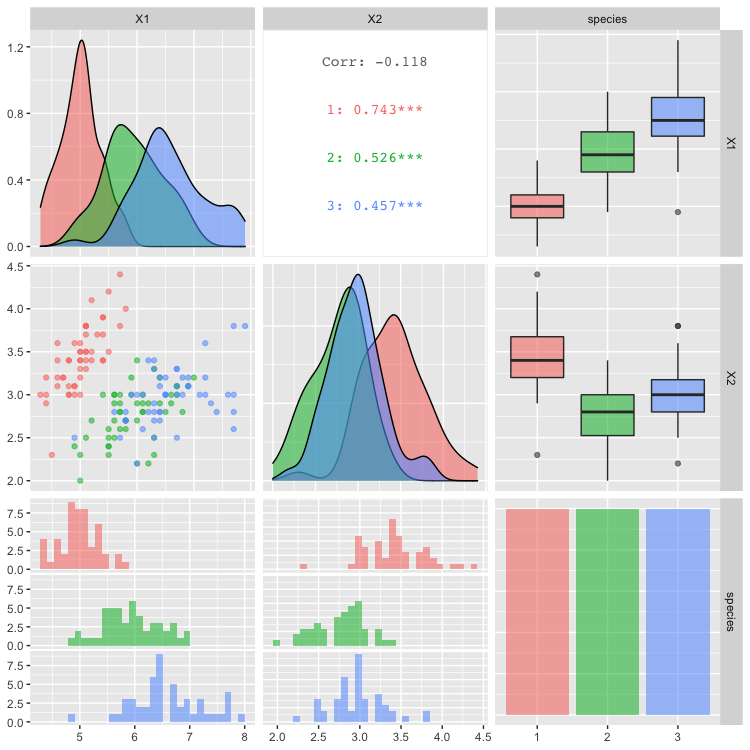
\includegraphics[width=3.0in]{I_1_matrix.png}
	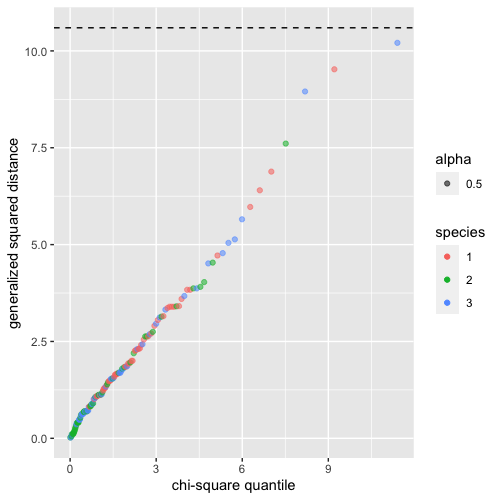
\includegraphics[width=3.0in]{I_1_chisq.png}
\end{center}

While there is no immediate indication of a departure from normality, a Box-Cox analysis of the bivariate distributions of each of the three species was performed to confirm the adequacy of normality. Contour plots for each of the three species show the surface of the likelihoods of an array of transformations on sepal length and sepal width. In each of the three plots, the point $(1,\ 1)$ lies near the maximum of the surface, suggesting again that no transformation of the data is necessary to fulfill normality.

\begin{center}
	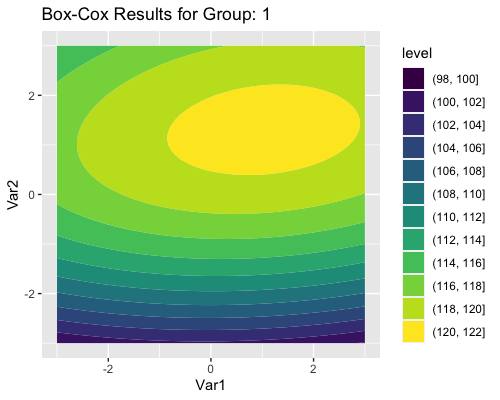
\includegraphics[width=2.0in]{I_1_bxcx.png}
	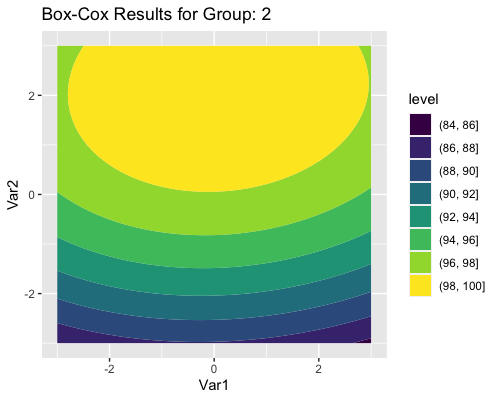
\includegraphics[width=2.0in]{I_2_bxcx.png}
	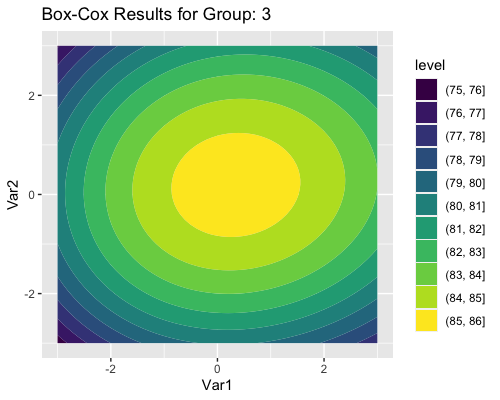
\includegraphics[width=2.0in]{I_3_bxcx.png}
\end{center}

\begin{enumerate}
\item[\bf{1-2.}]	
A multivariate analysis of variance, MANOVA, of the data was performed on the reduced data set (sepal length and sepal width only). The MANOVA is a method to identify differences in mean vectors across the three species. The hypothesis set is thus: $$H_0:\ \vec{\mu}_i = \vec{\mu}_j,\ H_0:\ \vec{\mu}_i \neq \vec{\mu}_j,\ i \neq j$$ The test statistic is formed from the MANOVA table via a measure called Wilk's Lambda, $\Lambda$. This measure is used to calculate a likelihood ratio test statistic defined as follows: $$\frac{n_1+n_2+n_3-3}{3-2} \cdot \frac{1-\Lambda^*}{\Lambda^*} \distras{} F_{3-1,\ n_1+n_2+n_3-3},\ \Lambda^* = \frac{\md{\mf{W}}}{\md{\mf{W} + \mf{B}}}$$

There are a basic set of assumptions that need validation prior to the MANOVA. The independent variables should be continuous and the dependent variables should be discrete (factors), and this is certainly the case. Observations should be independent of one another, and though we do not have information about the provenance of the data, it will be assumed that the measurements of one iris do not affect the measurements of another. As previously mentioned, the sample size for each species should be adequate with respect to the number of independent variables. The data should not contain any univariate or multivariate outliers, which has been previously established. Lastly, each of the species should exhibit homogeneity of sample covariance. This is established through the Bartlett test or via the Box-M test, which are calculated in R. The tests both suggest that homogeneity of sample covariance between the species is adequate.

\begin{center}
\begin{tabular}{| c  c  c |} 
	\hline
	test & statistic & p-value \\
	\hline
	&&\\
	Bartlett's K-squared & 2.0397 & 0.3607 \\
	&&\\
	Box-M & 0.9329 & 0.9880 \\
	&&\\
	\hline
\end{tabular}
\end{center}

The MANOVA table for the sample data is provided below. The calculated Wilk's Lambda statistic is $105.8788$ which exceeds the critical value of the $F$ distribution, $2.402$. This suggests that at least one of the pairs of mean vectors differ from one another.

\begin{center}
\begin{tabular}{|c c c |} 
	\hline
	Source of Variation & Matrix SSCP & degrees of freedom \\
	\hline
	&&\\
	Treatment & $\mf{B} = \m{63.212&-19.952\\-19.952&11.344}$ & $2$ \\
	&&\\
	Residual & $\mf{W} = \m{38.956&13.630\\13.630&16.962}$ & $147$ \\
	&&\\
	\hline
	&&\\
	Total (corrected) & $\mf{T} = \m{102.168&-6.322\\-6.322&28.306}$ & $149$ \\
	&&\\
	\hline
\end{tabular}
\end{center}

\item[\bf{3.}]	
	While the MANOVA results suggest at least one mean vector is significantly different from another, it does not provide any insight into which of the vector pairs differ nor to what degree. For now, let us consider only iris setosa and iris versicolor and see if their mean vectors differ. Denote the mean vector for setosa as $\vec{\mu}_1^{\intercal} = \m{\mu_{11} & \mu_{12}}$ and for versicolor as $\vec{\mu}_2^{\intercal} = \m{\mu_{21} & \mu_{22}}$. It is possible to filter the data set and rerun the MANOVA, but it is just as easy to conduct a Hotelling's $T^2$ test of the following hypothesis set: $$H_0: \vec{\mu}_1 = \vec{\mu}_2,\ H_a: \vec{\mu}_1 \neq \vec{\mu}_2$$ The same assumptions previously discussed should be inspected for this test. An identical set of tests performed in R do not suggest any violations of the assumptions, therefore we proceed with the test.

	The Hotelling $T^2$ test is defined as $$\m{\bar{X}_1 - \bar{X}_2}^{\intercal} \m{\p{\frac{1}{n_1} + \frac{1}{n_2}} \mf{S}_{pooled}} \m{\bar{X}_1 - \bar{X}_2} \distras{} \frac{\p{n_1+n_2-2}\cdot2}{n_1+n_2-2-1} \cdot F_{2,\ 97}$$ The calculated statistic is $498.5481$ which exceeds the critical value of the $F$ distribution given a confidence level of $\alpha = 0.05$, $\frac{98\cdot2}{97} F_{2,\ 97}^*(0.95)=6.2440$. Therefore, given the sample data, there is sufficient evidence to reject the null hypothesis, that is, one or both of sepal length and sepal width differs between iris setosa and iris versicolor.

	A $95\%$ confidence region for the difference between the means is given by the set: $$\{\vec{x}:\ \p{\vec{x}^{\intercal} - \m{-0.93 & 0.658}} \m{\p{\frac{1}{50} + \frac{1}{50}} \m{0.0078&0.0036\\0.0036&0.0048}} \p{\vec{x} -  \m{-0.93 \\ 0.658}} < 6.2440\}$$ This set of points define an ellipse whose half-axes are the eigenvectors of the pooled covariance matrix with lengths scaled to the square root of the respective eigenvector multiplied by the value on the right hand side of the equality.

\item[\bf{4.}]	
	The confidence region presented in part $\mf{I.3}$ was plotted for visualization in R. Along with the confidence ellipse, two sets of confidence intervals for both sepal length (X1) and sepal width (X2) are also drawn. The wider of the two sets of confidence intervals represents the simultaneous confidence interval which is equivalent to the projection of the confidence ellipse onto the respective axis. This is the more conservative of the two intervals. The narrower interval is the Bonferroni confidence interval, which is not scaled by the covariance between X1 and X2. In either case, the confidence region does not contain the point $(0,\ 0$, nor do either of the invervals contain the points $X1 = 0$ or $X2 = 0$. This suggests that there is a significant difference in both the sepal length and the sepal width of the two species. The numeric representation of the intervals is provided in a table below.

\begin{center}
	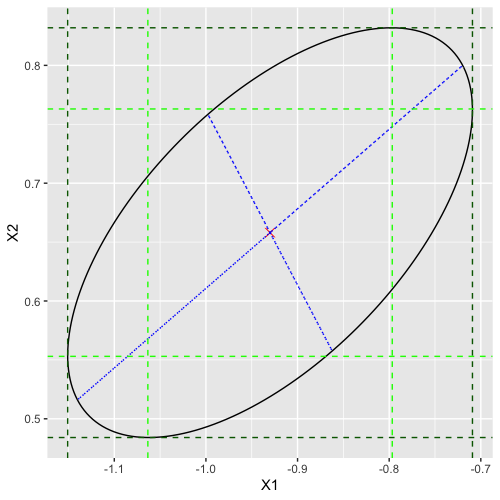
\includegraphics[width=3.0in]{I_4_ellipse.png}
\end{center}

\begin{center}
\begin{tabular}{| c c c c |} 
	\hline
	interval type & variable & lower confidence limit & upper confidence limit \\
	\hline
	&&&\\
	simultaneous & sepal length & -1.150 & -0.709 \\
	  & sepal width & 0.484 & 0.831 \\
	&&&\\
	\hline
	&&&\\
	Bonferroni & sepal length & -1.063 & -0.796 \\
	  & sepal width & 0.553 & 0.762 \\
	&&&\\
	\hline
\end{tabular}
\end{center}

\end{enumerate}

\newpage
\section*{Part 2}
	Throughout Part II, all of the data will be considered for the analysis. Previously, we confirmed the normal distribution of the sepal length (X3) and sepal width (X4). A similar analysis of the petal length and petal width is conducted below for use in future portions of the analysis. Note that given the visual analysis and the statistical tests (Wilks-Shapiro tests and normal correlation tests), there are possible violations of normality for X3 (see setosa) and X4 (see setosa and versicolor). Each of the three species was analyzed for ideal transformations to normality using the Box-Cox maximum likelihood method. Given the contour plots of the maximization surface, it is clear that X3 is the more problematic variable. The overall distribution (given all species combined) suggests a transformation is not necessary, however, when analyzed for each of the species, the suggested transformations are conflicting between species. Therefore, no transformation on the data will be pursued.

\begin{center}
	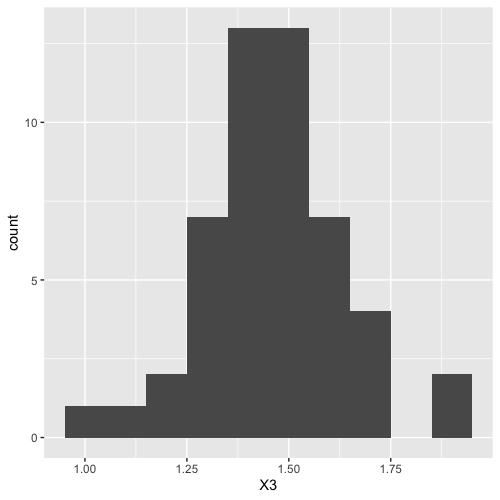
\includegraphics[width=1.5in]{II_1_X3_hist.png}
	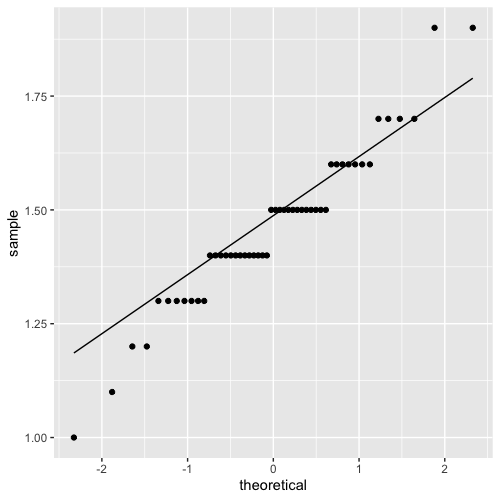
\includegraphics[width=1.5in]{II_1_X3_qq.png}
	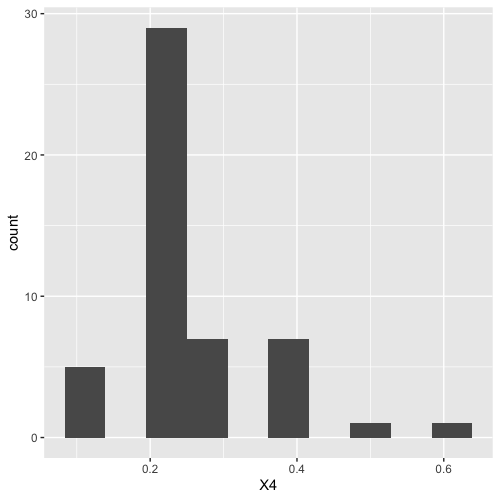
\includegraphics[width=1.5in]{II_1_X4_hist.png}
	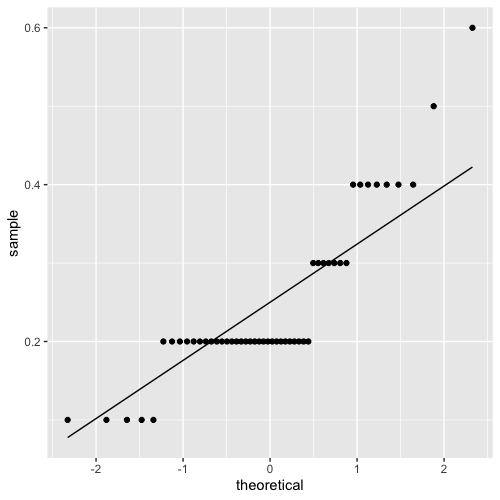
\includegraphics[width=1.5in]{II_1_X4_qq.png}
\end{center}
\begin{center}
	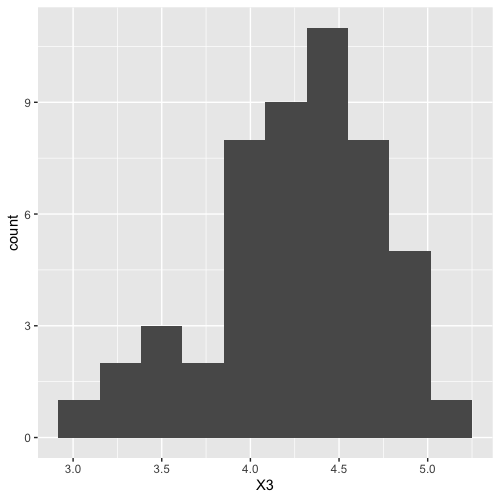
\includegraphics[width=1.5in]{II_2_X3_hist.png}
	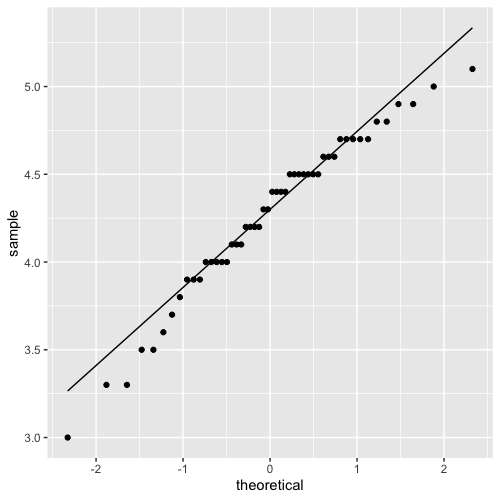
\includegraphics[width=1.5in]{II_2_X3_qq.png}
	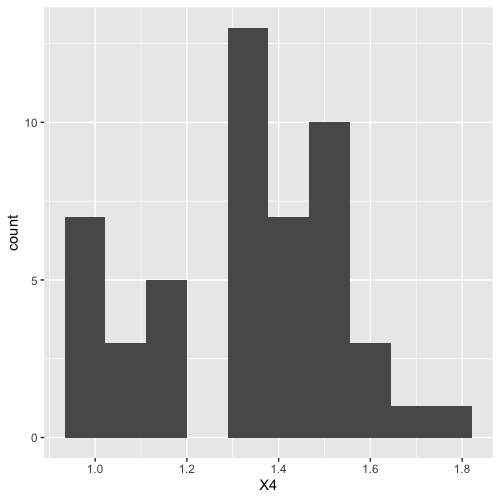
\includegraphics[width=1.5in]{II_2_X4_hist.png}
	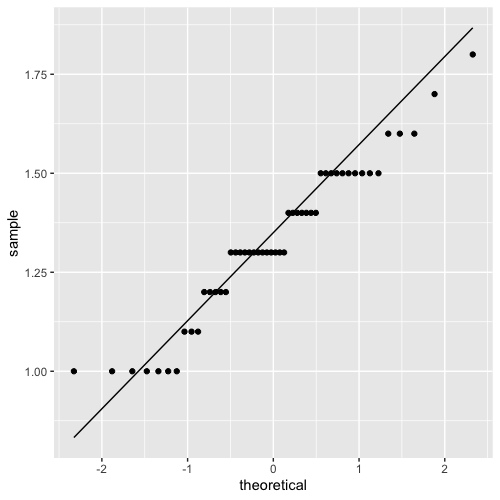
\includegraphics[width=1.5in]{II_2_X4_qq.png}
\end{center}
\begin{center}
	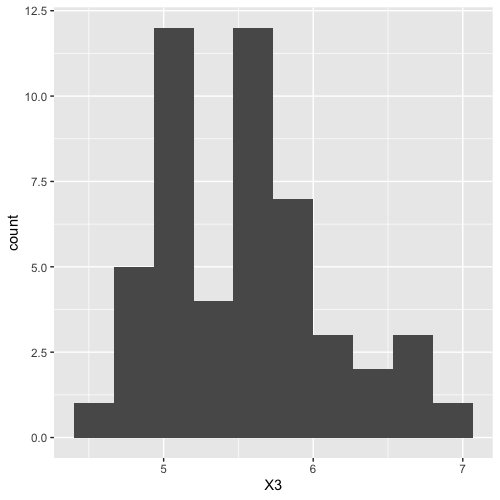
\includegraphics[width=1.5in]{II_3_X3_hist.png}
	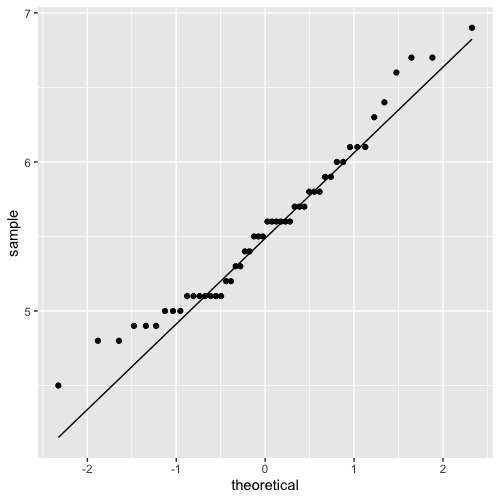
\includegraphics[width=1.5in]{II_3_X3_qq.png}
	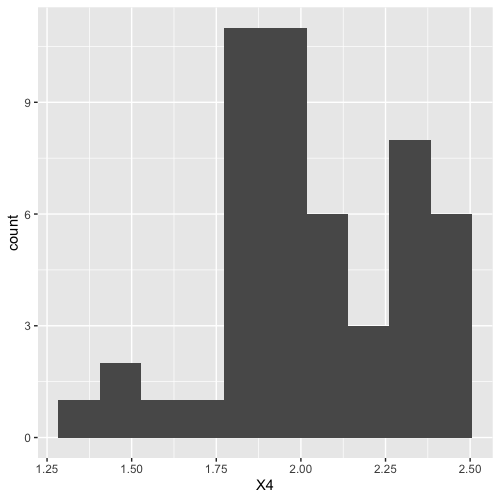
\includegraphics[width=1.5in]{II_3_X4_hist.png}
	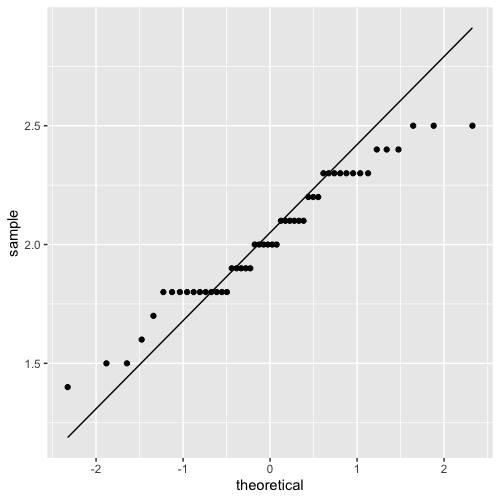
\includegraphics[width=1.5in]{II_3_X4_qq.png}
\end{center}

\begin{center}
\begin{tabular}{| c c | c c | c c |}
	\hline
	group & variable & Shapiro-Wilks & p-value & correlation test & p-value \\
	\hline
	&&&&&\\
	setosa & petal length & 0.954 & 0.054 & 0.974 & 0.032 \\
	& petal width & 0.799 & $<$0.001 & 0.891 & $<$0.001\\
	&&&&&\\
	versicolor & petal length & 0.966 & 0.158 & 0.983 & 0.161\\
	& petal width & 0.947 & 0.027 & 0.976 & 0.046 \\
	&&&&&\\
	virginica & petal length & 0.962 & 0.109 & 0.982 & 0.131 \\
	& petal width & 0.959 & 0.086 & 0.982 & 0.141 \\
	&&&&&\\
\hline
\end{tabular}
\end{center}

\begin{center}
	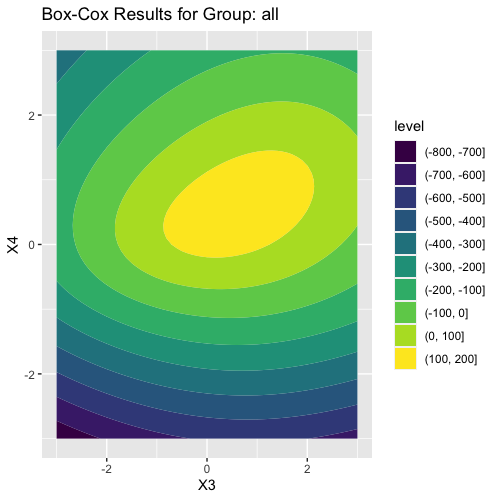
\includegraphics[width=1.5in]{II_all_bxcx.png}
	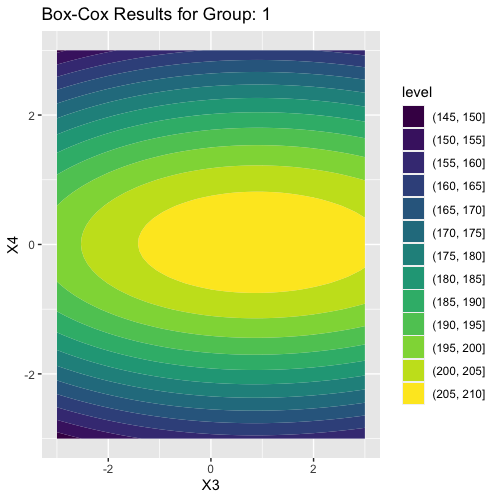
\includegraphics[width=1.5in]{II_1_bxcx.png}
	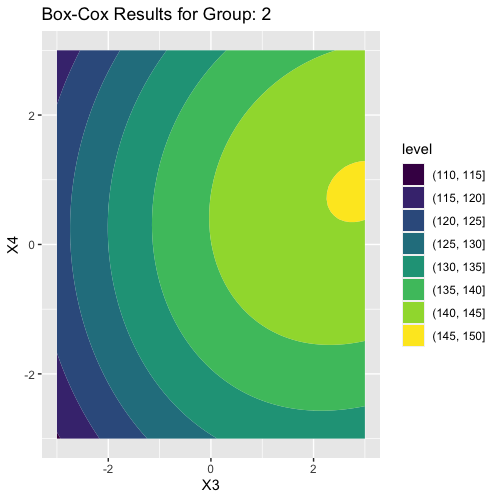
\includegraphics[width=1.5in]{II_2_bxcx.png}
	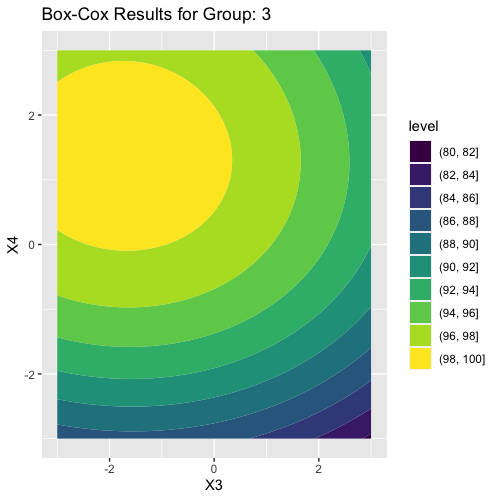
\includegraphics[width=1.5in]{II_3_bxcx.png}
\end{center}

	The bivariate distributions were observed via a scatterplot matrix on the four variables. Each of the bivariate spreads of data show roughly elliptical patterns when looked at by species. The updated generalized distance plot given all four variables support our original analysis on the first two variables. That is, there is no evidence of any generalized distances with extreme distances.
	
\begin{center}
	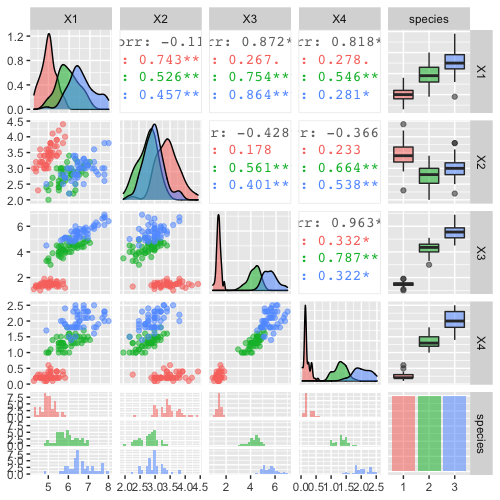
\includegraphics[width=3.0in]{II_matrix.png}
	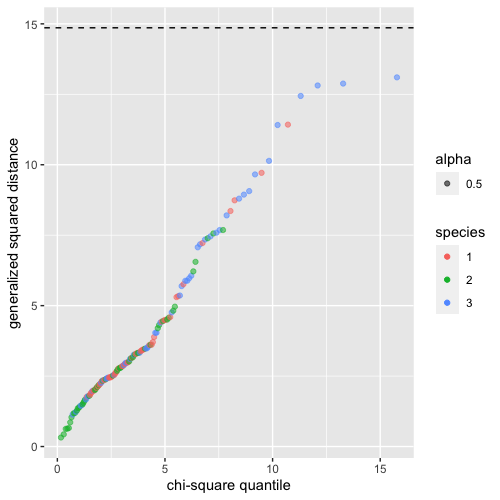
\includegraphics[width=3.0in]{II_chisq.png}
\end{center}

\newpage
\begin{enumerate}
\item[\bf{5.}]	
	A principal component analysis (PCA) of the data is now considered. The goal of PCA is to identify a reduced set of vectors that retain the variation of the sample data. The normality of the individual sample components is not required for PCA, only that a linear combination of the components is reasonable. Because the measurements on the flowers appear to belong to a similar range of values, a PCA on the sample covariance matrix was pursued. A PCA utilizes a spectral value decomposition of the covariance matrix. Because the sum of the eigenvalues of the covariance matrix is equivalent to the total sample variance, the proportion of variation explained by a set of the principal components is explained by the proportionate sum of the respective eigenvalues. A table of the eigenvalues and the cumulative sample variation accounted for is presented below. Additionally, a visual aid for selecting the correct number of principal components is providedby a scree plot. Both tools suggest that two principal components are adequate for representing the sample variation, which account for $97.7\%$ of the total variation.

\begin{center}
\begin{tabular}{|c c |}
	\hline
	eigenvalue & total proportion \\
	\hline
	4.228 & 0.924 \\
	0.242 & 0.977 \\
	0.078 & 0.994 \\
	0.023 & 1.000 \\
	\hline
\end{tabular}
\end{center}

\begin{center}
	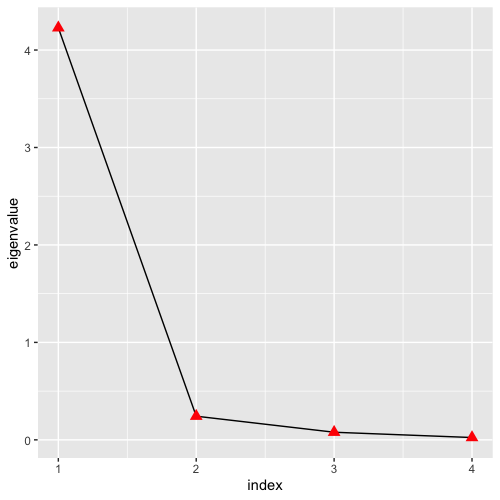
\includegraphics[width=1.75in]{II_5_scree.png}
	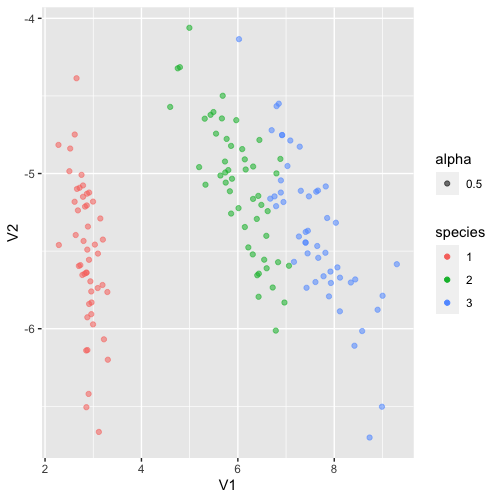
\includegraphics[width=1.75in]{II_5_scatter.png}
	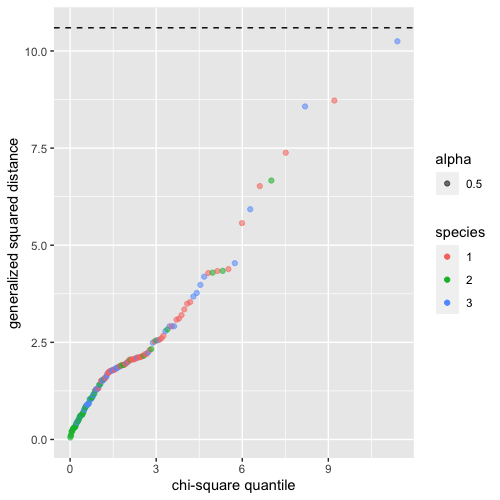
\includegraphics[width=1.75in]{II_5_chisq.png}
\end{center}

	A projection of the data into the bivariate representation by the first two principal components V1 and V2 is shown next to the scree plot. The first principal component is $(0.3613,\ -0.0845,\ 0.8566,\ 0.3582)$ and appears to represent the overall size of an iris. The second principal component is $(-0.6565,\ -0.7301,\ 0.1733,\ 0.0754)$ and provides a contrast between the sepal and petal measurements. The data is inspected for outliers using the generalized distance plot shown next to the scatter plot. It does not indicate any extreme values for any of the observations. Note also that the linearity of the plot is greatly improved, suggesting that the normality of the data may have improved after the projection. Again, the univariate normality of the projected is inspected. Histograms and quantile-quantile plots provide no evidence of a departure from nonnormality. Additionally, statistical tests for each of the groups support the adequacy of normality of the projected data.

\begin{center}
	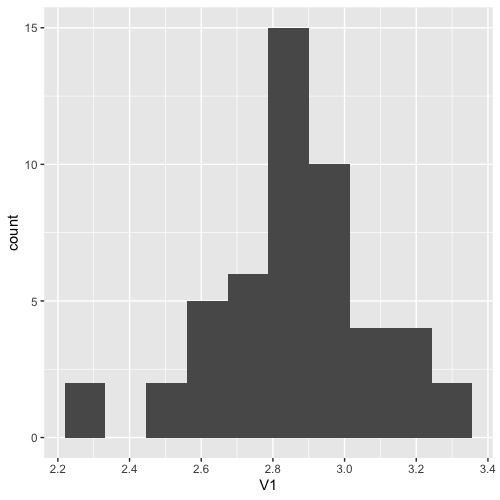
\includegraphics[width=1.4in]{II_1_V1_hist.png}
	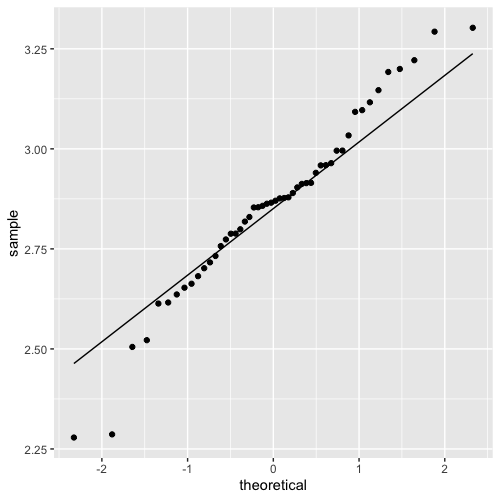
\includegraphics[width=1.4in]{II_1_V1_qq.png}
	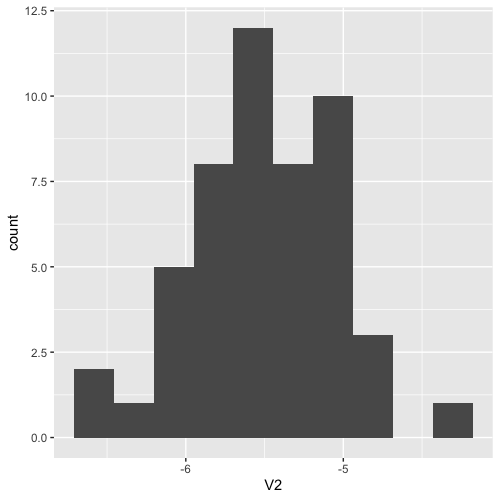
\includegraphics[width=1.4in]{II_1_V2_hist.png}
	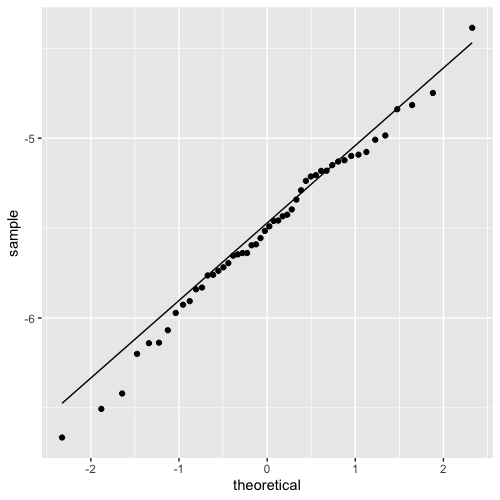
\includegraphics[width=1.4in]{II_1_V2_qq.png}
\end{center}
\begin{center}
	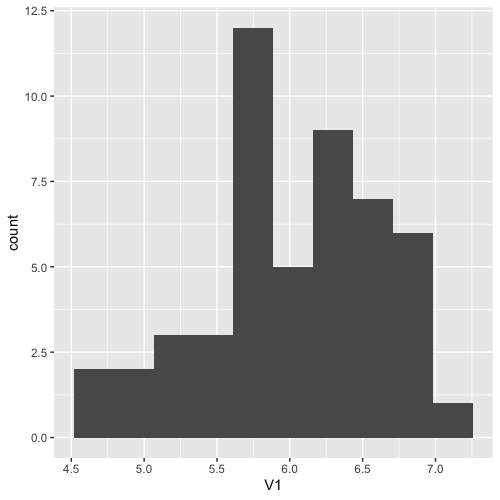
\includegraphics[width=1.4in]{II_2_V1_hist.png}
	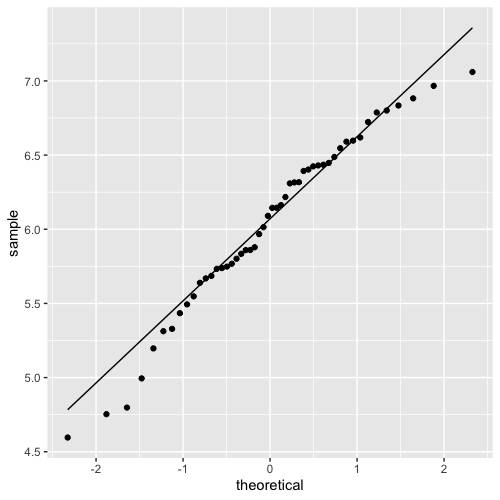
\includegraphics[width=1.4in]{II_2_V1_qq.png}
	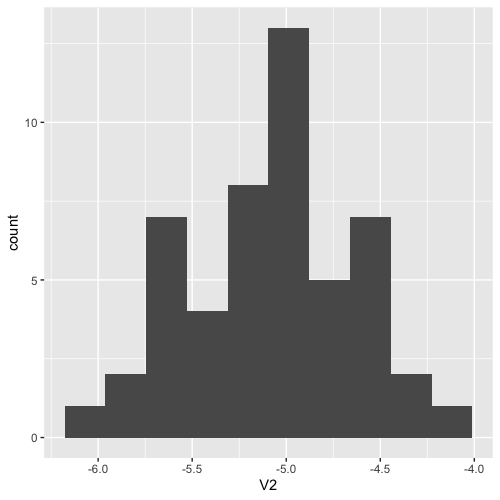
\includegraphics[width=1.4in]{II_2_V2_hist.png}
	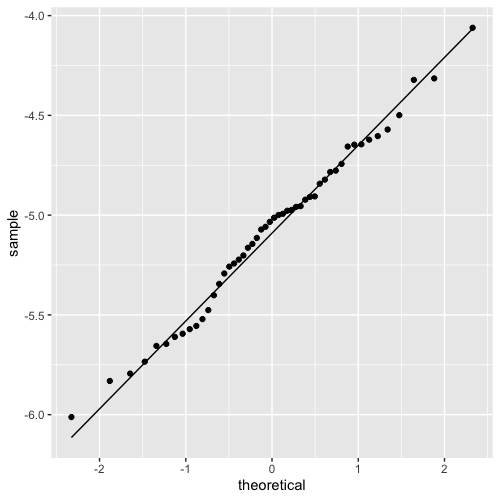
\includegraphics[width=1.4in]{II_2_V2_qq.png}
\end{center}
\begin{center}
	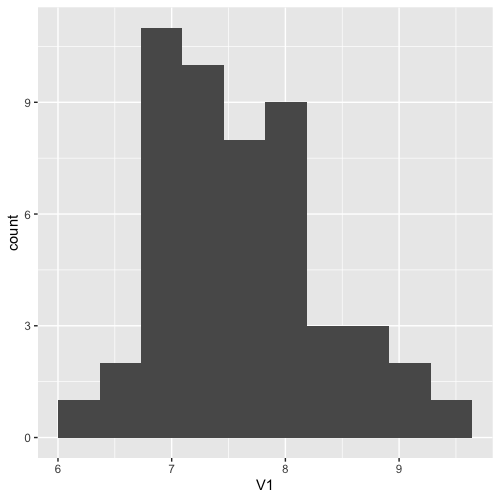
\includegraphics[width=1.4in]{II_3_V1_hist.png}
	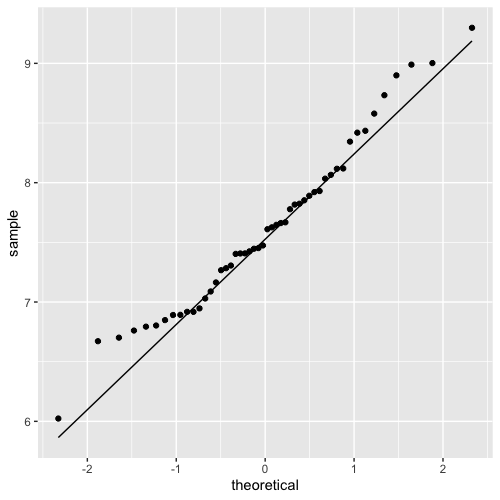
\includegraphics[width=1.4in]{II_3_V1_qq.png}
	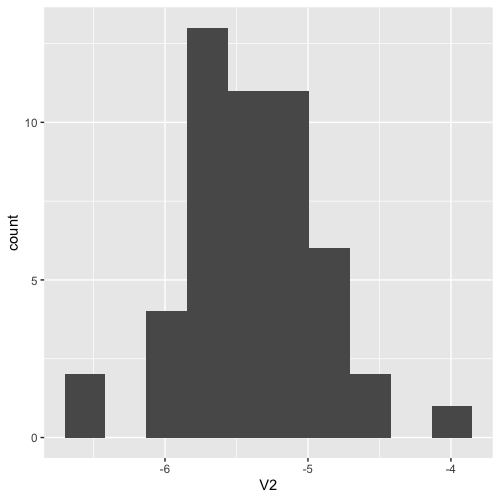
\includegraphics[width=1.4in]{II_3_V2_hist.png}
	\includegraphics[width=1.4in]{II_3_V2_qq.png}
\end{center}

	As a final measure to identify any potential outliers, a projection into the space spanned by the unused principal components was investigated. These projections should not contain any large component values. Fortunately, because there are only four variables in total, a graph of the projected values was also possible. The graph of the projections shows a randomly dispersed cloud of points, therefore, it is clear that there are no outliers in the originally projected data.

\begin{center}
	\includegraphics[width=3.0in]{II_5_altscatter.png}
\end{center}

\newpage
\item[\bf{6.}]	
	From Part II question $\bf{5}$, we found that a bivariate projection of the data given the first two principal components was sufficient for capturing the a majority of variation from the original sample data with all four iris measurements. It was also clear that after projecting the groups, the groups were separated reasonably well, with some overlap between species versicolor and virginica. Utilizing the data projected by the principal components, we now seek to develop a classification rule for the three iris species. From the prior analysis, it is clear that the projected data are approximately normal within each species. Extending this analysis, a Box-M test as well as a Bartlett test were performed. They establish that the three species also exhibit homogeneity of covariance. This allows us to utilize the minimized expected cost of misclassification for multiple groups with equal covariance to establish the classification rule.
	
	Because the sample size of each group is equal, and because no outliers were identified after projecting the data via the principal components, the prior probabilities for each of the three species are equal, that is $p_i = \frac{1}{3},\ i = 1,\ 2,\ 3$. Furthermore, we will assume that the cost of misclassifying an observation that belongs to population k ($\pi_k$) to population i, given by $c(k|i)$, are equal for all possible misclassifications. In general, the classification rule ($R_k$) for allocating a vector ($\vec{x}$) to $\pi_k$ is given by: $$R_k :\ \sum_{i \neq k}^{g} p_i \cdot f_i(\vec{x}) \cdot c(k|i) \leq \sum_{i \neq j}^{g} p_i \cdot f_i(\vec{x}) \cdot c(j|i),\ j = 1, \ldots, g,\ j \neq k$$ However, in this case, all misclassification costs are equal, therefore the k-th classification rule can be simplified to: $$R_k:\ p_k \cdot f_k(\vec{x}) \geq p_i \cdot f_i(\vec{x})$$

	Given the projected sample data is normal and that it exhibits homogeneity of covariance between species, it is possible to utilize a linear discriminant score that will lead to classification decisions for a given observation. The sample version of the linear discriminant score is given by: $$\hat{d}_i \p{\vec{x}} = \hat{\vec{x}}_i^{\intercal} \mf{S}_{pooled}^{-1} \vec{x} - \frac{1}{2} \hat{\vec{x}}_i^{\intercal} \mf{S}_{pooled}^{-1} \hat{\vec{x}}_i + ln\p{p_i}$$. Then, assign $\vec{x}$ to $\pi_k$ if $\hat{d}_k \p{\vec{x}} = max \hat{d}_i \p{\vec{x}},\ i = 1,\ 2,\ 3$. These scores were computed in R and appended to the data. A portion of the data is printed below.

\begin{rc}

# A tibble: 150 x 8
       V1    V2 species    d_1   d_2       d_3 class correct
    <dbl> <dbl> <fct>    <dbl> <dbl>     <dbl> <int> <lgl>  
  1  2.82 -5.65 1        87.8   42.8   5.81        1 TRUE   
  2  2.79 -5.15 1        70.5   35.4   1.03        1 TRUE   
  3  2.61 -5.18 1        73.7   33.8  -2.26        1 TRUE   
  4  2.76 -5.01 1        65.9   33.1  -0.787       1 TRUE   
  5  2.77 -5.65 1        88.6   42.4   4.97        1 TRUE   
  6  3.22 -6.07 1        98.2   53.5  17.6         1 TRUE   
  7  2.68 -5.24 1        74.9   35.4  -0.396       1 TRUE   
  8  2.88 -5.49 1        81.6   41.3   5.68        1 TRUE   
  9  2.62 -4.75 1        58.3   27.7  -5.84        1 TRUE   
 10  2.83 -5.21 1        72.3   36.8   2.41        1 TRUE   

...

139  6.67 -5.16 3        26.8   81.1  80.2         2 FALSE  
140  7.61 -5.70 3        35.3   99.7 104.          3 TRUE   
141  7.82 -5.51 3        26.2   99.5 106.          3 TRUE   
142  7.42 -5.74 3        38.7   98.1 100.          3 TRUE   
143  6.92 -4.75 3         9.50  78.2  81.8         3 TRUE   
144  8.07 -5.60 3        26.7  104.  112.          3 TRUE   
145  7.92 -5.63 3        29.3  102.  110.          3 TRUE   
146  7.45 -5.51 3        30.6   95.2  98.9         3 TRUE   
147  7.03 -4.95 3        15.3   82.3  85.7         3 TRUE   
148  7.27 -5.41 3        28.7   91.5  94.4         3 TRUE   
149  7.40 -5.44 3        28.5   93.7  97.5         3 TRUE   
150  6.89 -5.04 3        20.2   82.0  83.7         3 TRUE 

\end{rc}

	Along with the linear discriminant scores, the suggested classification and whether that classification was correct were also added as columns to the dataset. With that information collected, it is easy to construct a confusion matrix and obtain the apparent error rate (APER) of the classification. The sums of the rows of the confusion matrix represent the sample counts for each species. The diagonal elements of the confusion matrix represent appropriately classified irises, whereas the off-diagonal elements represent misclassified irises. The apparent error rate of classification is obtained by taking the sum of the off-diagonal elements as the numerator and the sum of the row margins (total sample size) as the denominator. Given this classification, the estimated actual error rate (AER) is $\frac{6}{150} = 0.04$, or $4\%$.

\begin{center}
\begin{tabular}{| c | c | c c c |}
	\hline
	&& & predicted class & \\
	\hline
	&& setosa & versicolor & virginica \\
	\hline
	&&&&\\
	& setosa& 50 & 0 & 0 \\
	&&&&\\
	&&&&\\
	actual class & versicolor & 0 & 48 & 2 \\
	&&&&\\
	&&&&\\
	& virginica & 0 & 4 & 46 \\
	&&&&\\
	\hline
\end{tabular}
\end{center}

If a new observation was collected and the measurements given were $(6.7, 2.5, 5.8, 1.8)'$, the classification rule would assign the iris as follows. First, the measurements are projected via the principal components used previously. The resulting projected vector is $(7.823, -5.083)'$. Next, the linear discriminant scores for setosa, versicolor, and virginica, are $8.767$, $91.282$, and $100.784$, respectively. Therefore, the new observation should be appropriately classified to the virginica species. Adding this observation to the scatterplot of the projections, we find that the classification appears commensurate to our previous observations. The new observation is represented by a large triangle on the scatterplot.

\begin{center}
	\includegraphics[width=5.0in]{II_6_scatter.png}
\end{center}


\end{enumerate}

\end{document}
